\section{Homothetic family}

The family of 3-periodics interscribed in a pair of homothetic ellipses is depicted in \cref{fig:06-six-caps}(bottom left). Let $a,b$ be the semi-axes of the outer ellipse. The Cayley condition for this pair implies that $a_c=a/2$ and $b_c=b/2$, see  \cref{prop:03-homothetic-cayley}.

Recall the barycenter $X_2$ is stationary at the common center and the area $A=(3 a b \sqrt{3})/{4}$ is invariant.

Recall that over the confocal family, the locus of the incenter $X_1$ (resp. symmedian point $X_6$) was an ellipse (resp. a quartic). Teferring to \cref{fig:06-homoth-x1x6}, this is reversed in the homothetic family: 

\begin{proposition}
Over homothetic 3-periodics, the locus of the incenter $X_1$ (resp. symmedian point $X_6)$ is a quartic (resp. an ellipse). These are given by:

\begin{align*}
\text{locus of $X_1$}: \;& 
16\, \left( {a}^{2}{y}^{2}+{b}^{2}{x}^{2} \right)  \left( {a}^{2}{x}^{
2}+{b}^{2}{y}^{2} \right) -8\,{b}^{2} \left( {a}^{4}+5\,{a}^{2}{b}^{2}
+2\,{b}^{4} \right) {x}^{2}\\
&-8\,{a}^{2} \left( 2\,{a}^{4}+5\,{a}^{2}{b}
^{2}+{b}^{4} \right) {y}^{2}+{a}^{2}{b}^{2} \left( a^2-b^2 \right) ^{2}=0,
 \\
\text{locus of $X_6$}: &\; \frac{x^2}{a_6^2}+\frac{y^2}{b_6^2}=1,\;a_6=\frac{a(a^2-b^2)}{2(a^2+b^2)},\;\;\; b_6=\frac{b(a^2-b^2)}{2(a^2+b^2)} \cdot\\
\end{align*}
\label{prop:06-homoth-x1x6}
\end{proposition}

\begin{figure}
    \centering
    \includegraphics[width=.7\textwidth]{chap_06/pics/pics_06_040_homoth_x16.png}
    \caption{A homothetic 3-periodic and the quartic (resp. elliptic) locus of the incenter $X_1$ (resp. symmedian point $X_6$). \href{https://bit.ly/3oR5nCN}{Live}}
    \label{fig:06-homoth-x1x6}
\end{figure}

\begin{proof}
CAS-assisted simplification.
\end{proof}

\subsection{Four Circular Loci}

The two Fermat points $X_{13}$ and $X_{14}$ as well as the two isodynamic points $X_{15}$ and $X_{16}$ have trilinear coordinates which are irrational on the sidelengths of a triangle, see \cite{etc}. Indeed, over billiard 3-periodics, their loci are non-elliptic.

Referring to \cref{fig:06-homoth-circ-loci}:

\begin{proposition}
Over homothetic 3-periodics, the loci of $X_k$, $k=$13,14,15,16 are four distinct circles. Their radii are $(a-b)/2$, $(a+b)/2$, $(a-b)^2/z$, and $(a+b)^2/z$, respectively, where $z=2(a+b)$.
\label{prop:06-homoth-four-circles}
\end{proposition}

\begin{figure}
    \centering
    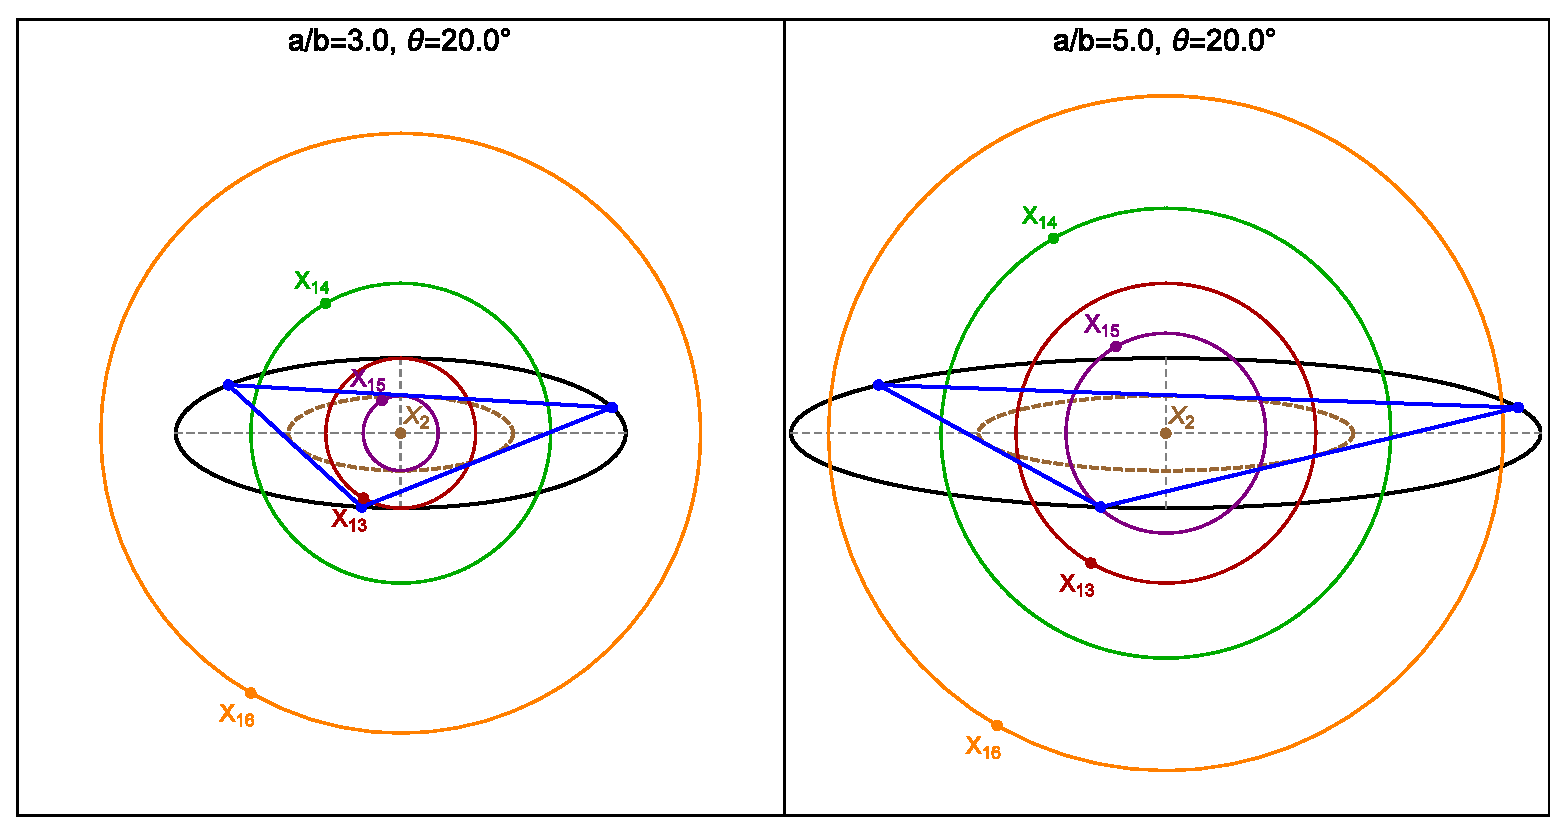
\includegraphics[width=\textwidth]{pics_06_050_system_III_circular_loci.eps}
    \caption{Circular loci of the first and second Fermat points $X_{13}$ and $X_{14}$ (red and green) as well as the first and second isodynamic points $X_{15}$ and $X_{16}$ (purple and orange) for two aspect ratios of the homothetic pair: $a/b=3$ (left) and $a/b=5$ (right). The radius of the $X_{16}$ locus is minimal at the first case. \href{https://youtu.be/ZwTfwaJJitE}{Video}, \href{https://bit.ly/3yF0wc9}{Live}}
    \label{fig:06-homoth-circ-loci}
\end{figure}